\subsubsection{Детектирование слабого сигнала с помощью осциллятора Дуффинга}
\label{ssec:duffing}

Теория колебаний и волн возникла примерно в 18 веке. Ее началом принято считать труды Лагранжа, опубликованные в 1788 г. Введя обобщенные
координаты и импульсы, Лагранж, отошел от традиционной механики и записал динамические уравнения, которые могут быть отнесены к системам
любой природы. Подробную историю возникновения теории колебаний и волн можно найти во введении к \cite{landa_book}. 
Введем некоторые используемые в работе термины.

\emph{Аттрактором} называется множество точек в фазовом пространстве, к которому стремятся со
временем все соседние фазовые траектории из некоторой области, называемой областью притяжения \cite{landa_book}.

\emph{Динамической системой} называют такую систему, движение которой задается набором правил. Для динамической системы можно ввести
понятие \emph{состояние}, определяемого набором величин, называемых \emph{динамическими переменными}.

\emph{Фазовое пространство} - пространство динамических переменных, полностью определяющих состояние системы.

\emph{Ляпуновский показатель} - 
характеризует степень расходимости близких фазовых траекторий, и число положительных ляпуновских показателей, характеризующее число направлений
неустойчивости. Максимальный ляпуновский показатель:
\begin{center}
\begin{equation}
	\label{eq:exp_lyapunova_1}
	\lambda = \lim_{\substack{t \to \infty\\d \to 0}}\ln \frac{d(t)}{d(0)},
\end{equation}
\end{center}
где ${d(t)}$ - расстояние между двумя близкими фазовыми траекториями. Непосредственный рассчет показателей по данной формуле является
затруднительным для систем с экспененциальной неустойчивостью траектории. В \cite{landa_book} рассмотрен более простой способ:
\begin{center}
\begin{equation}
	\label{eq:exp_lyapunova_2}
	\lambda = \frac{1}{m}\sum \limits_{i=1}^m \lambda_i = \frac{1}{m\tau}\ln\prod \limits_{i=1}^md_i,
\end{equation}
\end{center}
где локальный ляпуновский показатель ${\lambda_i}=(1/ \tau)\ln d_i$, ${d_i}$ - отношение расстояние между траекториями в конце ${i}$ - го
шага к начальному расстоянию, ${\tau}$ - длительность промежутка.

Динамическая система описываемая уравнением \ref{eq:oscillator_basic} на двумерной фазовой плоскости называется - осциллятором (система
описываемая на двумерном фазовом цилиндре - ротаторе в данной работе не рассматривается)\cite{chaos_neimark_landa}.
\begin{center}
\begin{equation}
	\label{eq:oscillator_basic}
	x'' + 2\delta(x, x') + Q(x) = 0
\end{equation}
\end{center}

Частным случаем уравнения \ref{eq:oscillator_basic} является уравнение Дуффинга, которое описывает явление нелинейного резонанса:
\begin{center}
\begin{equation}
	\label{eq:oscillator_duffing}
	x'' + 2\delta{x'} + ax +bx^3 = F\cos{\nu{t}}
\end{equation}
\end{center}

Детектирование сигналов с расширенным спектром (в частности сигналов системы Navstar GPS) с помощью осциллятора Дуффинга
достаточно новое направление в исследованиях по данной тематике. В частности
\cite{chaos_chen, chaos_cambridge, chaos_huang, chaos_song}. Так же является интересной более ранняя статья не рассматривающая GPS
\cite{chaos_wang}.

Осциллятор Дуффинга с периодическим внешним воздействием может быть описан уравнением:
\begin{center}
\begin{equation}
	\label{eq:duffing}
	mx'' + cx' + k_{1}x + k_{2}x^3 = F_{0}\cos(\omega{t})
\end{equation}
\end{center}

где
$m$- масса,
$c$ - коэффициент диссипации,
$x$ - состояние осциллятора,
$k_1$ и $k_2$ - линейный и нелинейный коэффициенты соответственно.
$F_{0}\cos(\omega{t})$ - внешнее воздействие.

Подробно уравнение \ref{eq:duffing} рассмотрено в \cite{chaos_neimark_landa} (Глава 9 параграф 3).
Для использования осциллятора Дуффинга для детектирования сигналов системы GPS была предложена
усовершенствованная форма \cite{chaos_song, chaos_chen}:
\begin{center}
\begin{equation}
	\label{eq:duffing_gps}
	x'' +cx' - x^3 + x^5 = \gamma\cos(\omega{t}) + (\gamma_{x}\cos(\omega_{x}) + n(t))
\end{equation}
\end{center}

Перепишем динамическую систему \ref{eq:duffing_gps} в виде:
\begin{center}
\begin{eqnarray}
	\label{eq:duffing_gps_2}
	y(t) & = & x'(t) \\
	y'(t) & = & -cx' + x^3 - x^5 + \gamma\cos(\omega{t}) + (\gamma_{x}\cos(\omega_{x}) + n(t))
\end{eqnarray}
\end{center}

Пример фазового портрета при ${\omega=\omega_{x}}$ изображен на рисунке \ref{pic:duffing_sync},
фазовый портрет хаоса расположен на рисунках \ref{pic:duffing_chaos1}, \ref{pic:duffing_chaos2}
\begin{figure}[H]
	\center\scalebox{0.5}{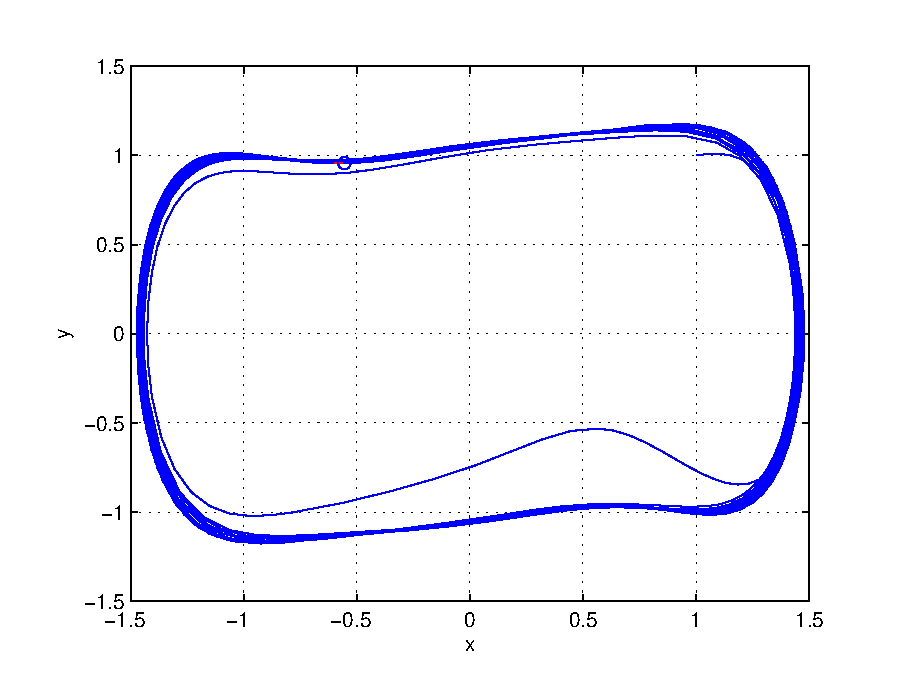
\includegraphics[width=1\linewidth]{duffing_sync.eps}}
	\caption{Фазовый портрет при ${\omega =\omega_{x}}$}
	\label{pic:duffing_sync}
\end{figure}

\begin{figure}[H]
	\center\scalebox{0.5}{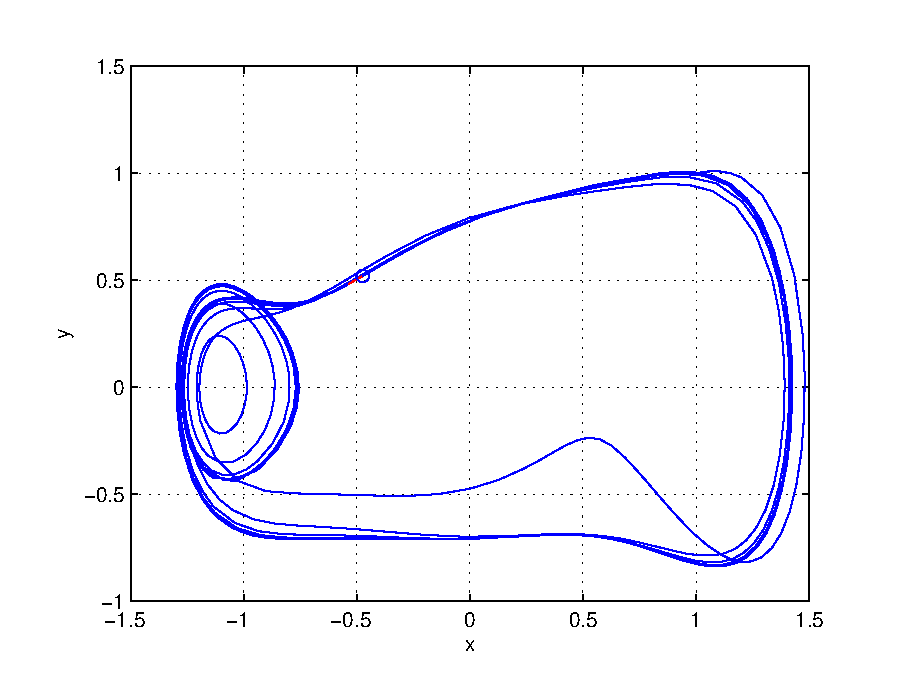
\includegraphics[width=1\linewidth]{duffing_chaos1.eps}}
	\caption{Фазовый портрет при ${\omega < \omega_{x}}$}
	\label{pic:duffing_chaos1}
\end{figure}

\begin{figure}[H]
	\center\scalebox{0.5}{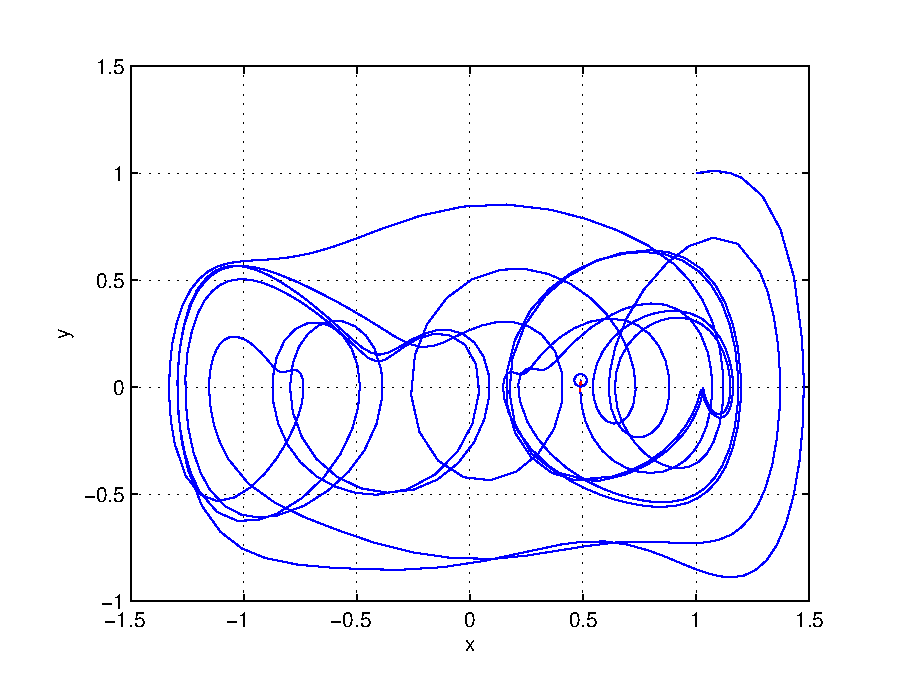
\includegraphics[width=1\linewidth]{duffing_chaos2.eps}}
	\caption{Фазовый портрет при ${\omega > \omega_{x}}$}
	\label{pic:duffing_chaos2}
\end{figure}

В качестве параметров уравнения применялись $c = 0.5$, $\gamma=\gamma_{x}=0.36$, ${\omega=1}$

Часто для вычисления характеристик хаотической динамики применяется показатель Ляпунова.
Он показывает в каком состоянии находится система. Если система находится
в стабильном состоянии линии фазовой траектории будут близко прилегать одна к другой, в противном
случае система находится в состоянии хаоса. Детектор с применением показателя ляпунова
представлен на рисунке \ref{pic:chaos_lyapunov}.

\begin{figure}[H]
	\center\scalebox{0.7}{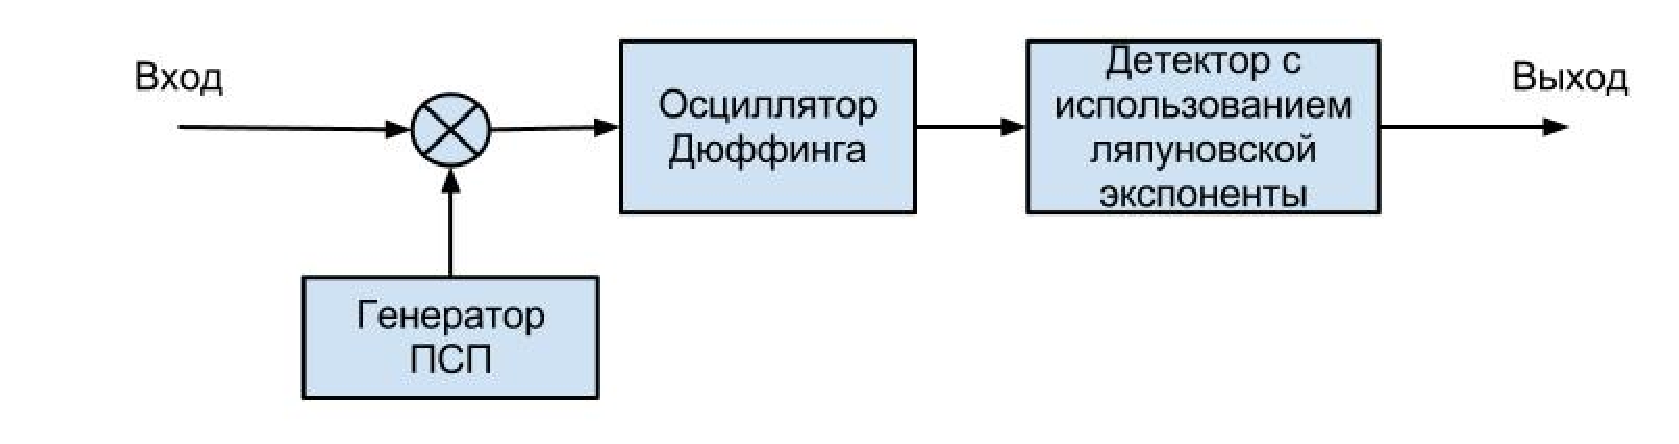
\includegraphics[width=1\linewidth]{Chaos_detector_Lyapunov.eps}}
	\caption{Схема детектора основанного на показателе ляпунова для осциллятора Дуффинга}
	\label{pic:chaos_lyapunov}
\end{figure}

В статье \cite{chaos_chen} предложен усовершенствованный метод, базирующийся на вычислении дисперсии
фазовой траектории. Действительно, на рисунках \ref{pic:duffing_sync}, \ref{pic:duffing_chaos1},
\ref{pic:duffing_chaos2} видно - когда система находится в хаотическом состоянии значение
дисперсии по координате ${x}$, чем соответствующее значение в состоянии $\omega = \omega_{x}$.
На основе этого была предложена усовершенствованная схема детектора сигнала
\ref{pic:chaos_energy_detector}

\begin{figure}[H]
	\center\scalebox{0.7}{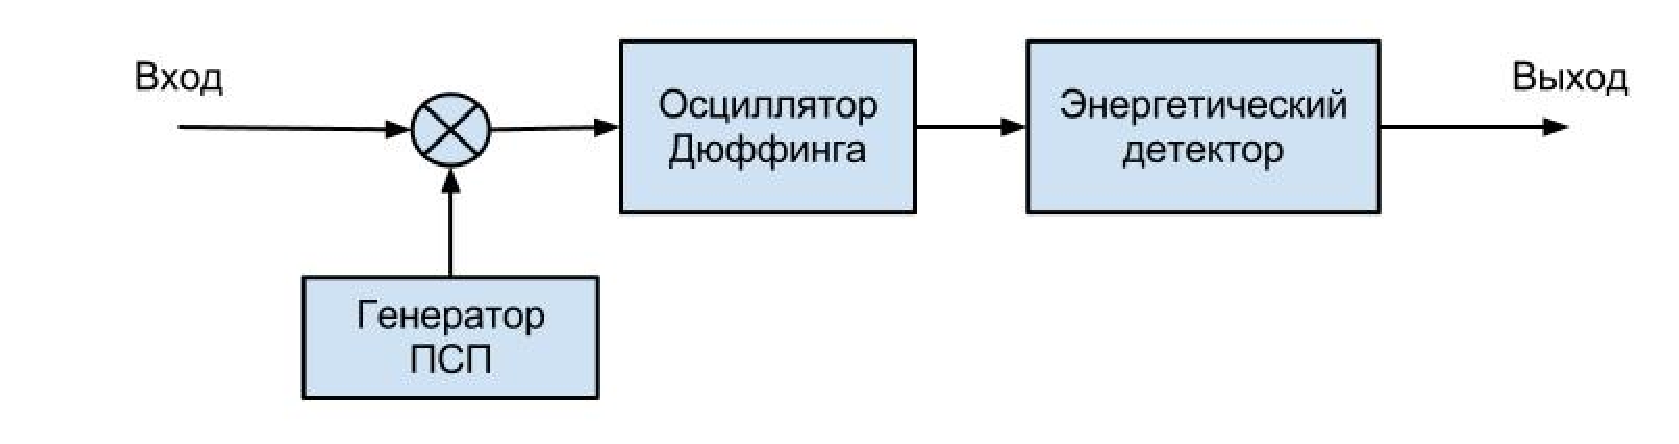
\includegraphics[width=1\linewidth]{chaos_detector.eps}}
	\caption{Схема энергетического детектора для осциллятора Дуффинга}
	\label{pic:chaos_energy_detector}
\end{figure}

\newpage
